The constant $c_s$ model was chosen as the model to test PTtools with, as the model is relatively simple and there is some reference data available from \cites{giese_2020}{giese_2021}.
Figure \ref{fig:fluid_profiles} demonstrates solutions for three different wall speeds $v_\text{wall}$ and $\alpha_n$.
These are the same values as in \cite[fig. 10]{hindmarsh_gw_pt_2019}.
However, instead using only the bag model $c_{s,s}^2 = c_{s,b}^2 = \frac{1}{3}$,
we consider the four different combinations of the speeds of sound
$c_{s,s}^2 \in \{ \frac{1}{3}, \frac{1}{4} \}, c_{s,b}^2 \in \{ \frac{1}{3}, \frac{1}{4} \}$.

\begin{figure}[h!]
\centering
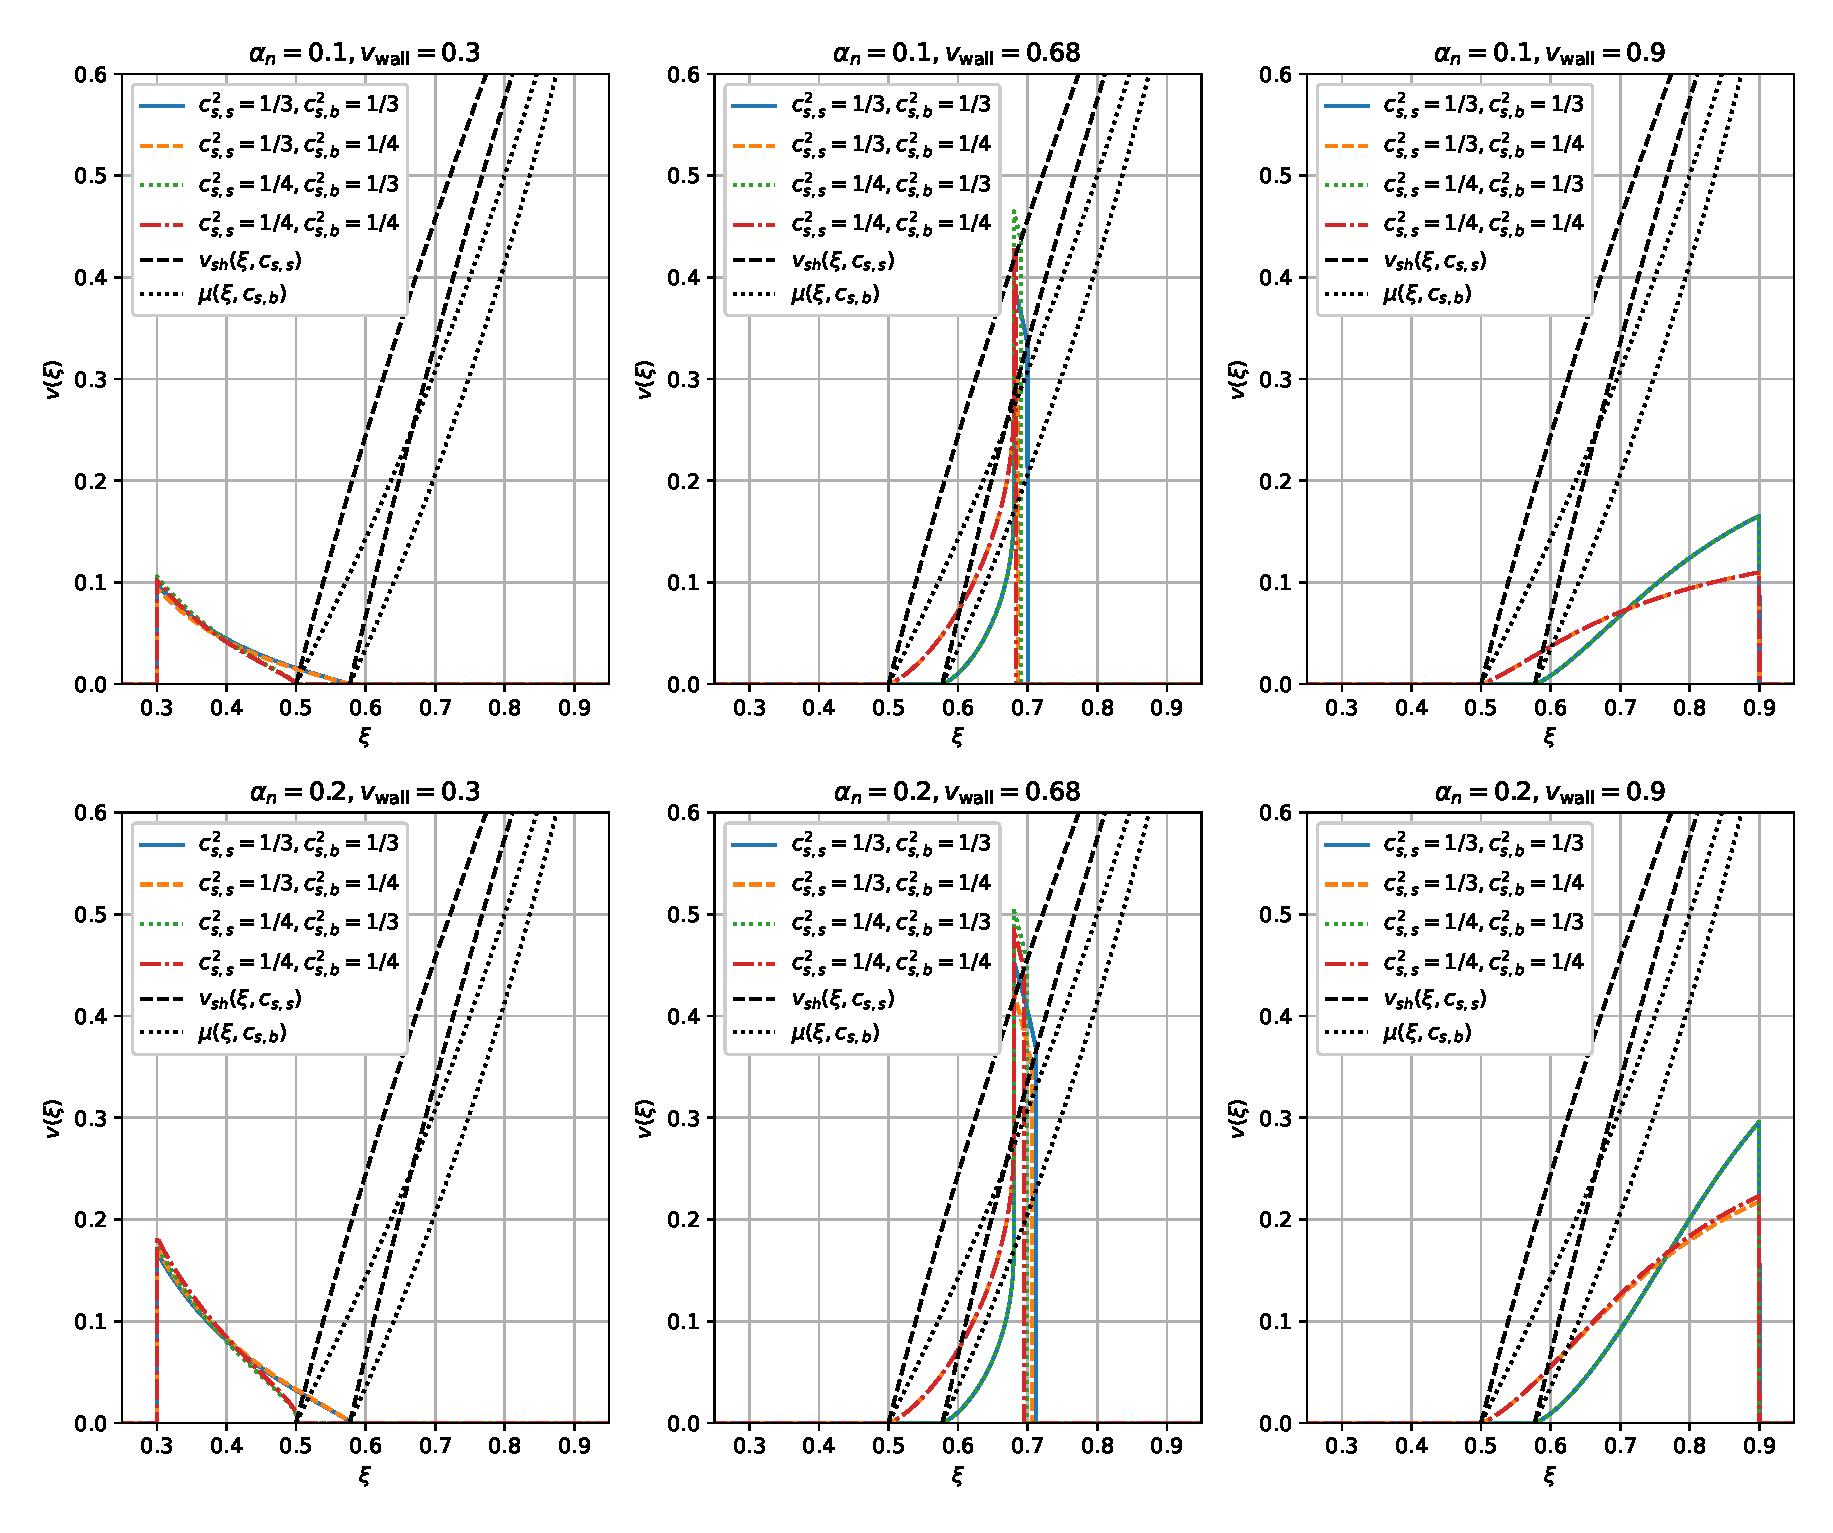
\includegraphics[width=\textwidth]{../pttools/examples/fig/const_cs_gw_v.eps}
\caption{Self-similar fluid profiles}
\label{fig:fluid_profiles}
\end{figure}

\begin{figure}[h!]
\centering
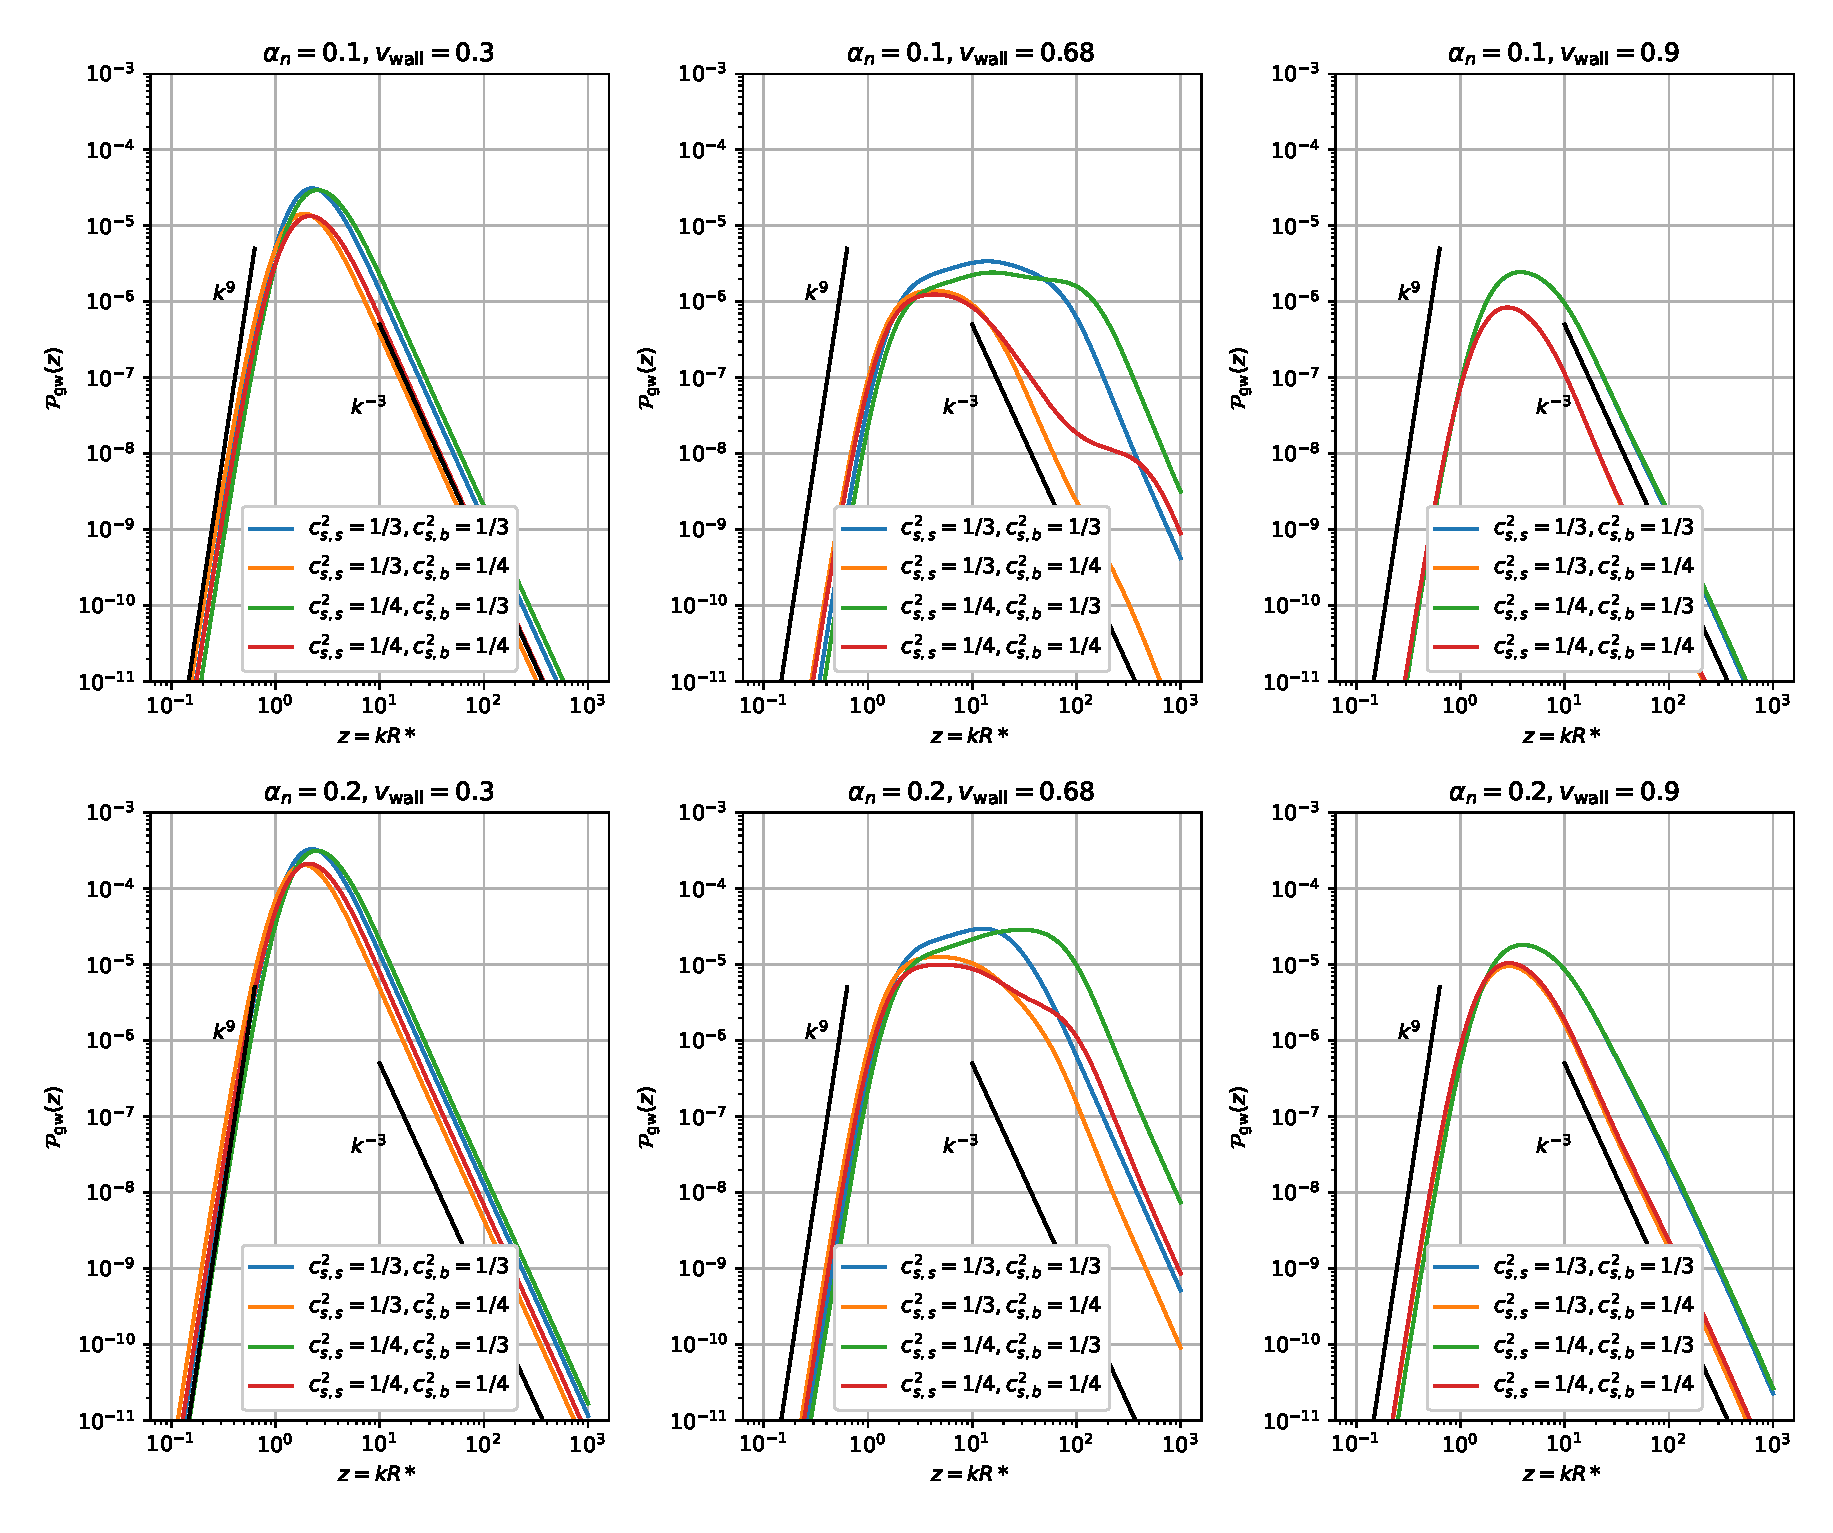
\includegraphics[width=\textwidth]{../pttools/examples/fig/const_cs_gw.eps}
\caption{Gravitational wave power spectra}
\label{fig:gw_spectra}
\end{figure}

\begin{figure}[h!]
\centering
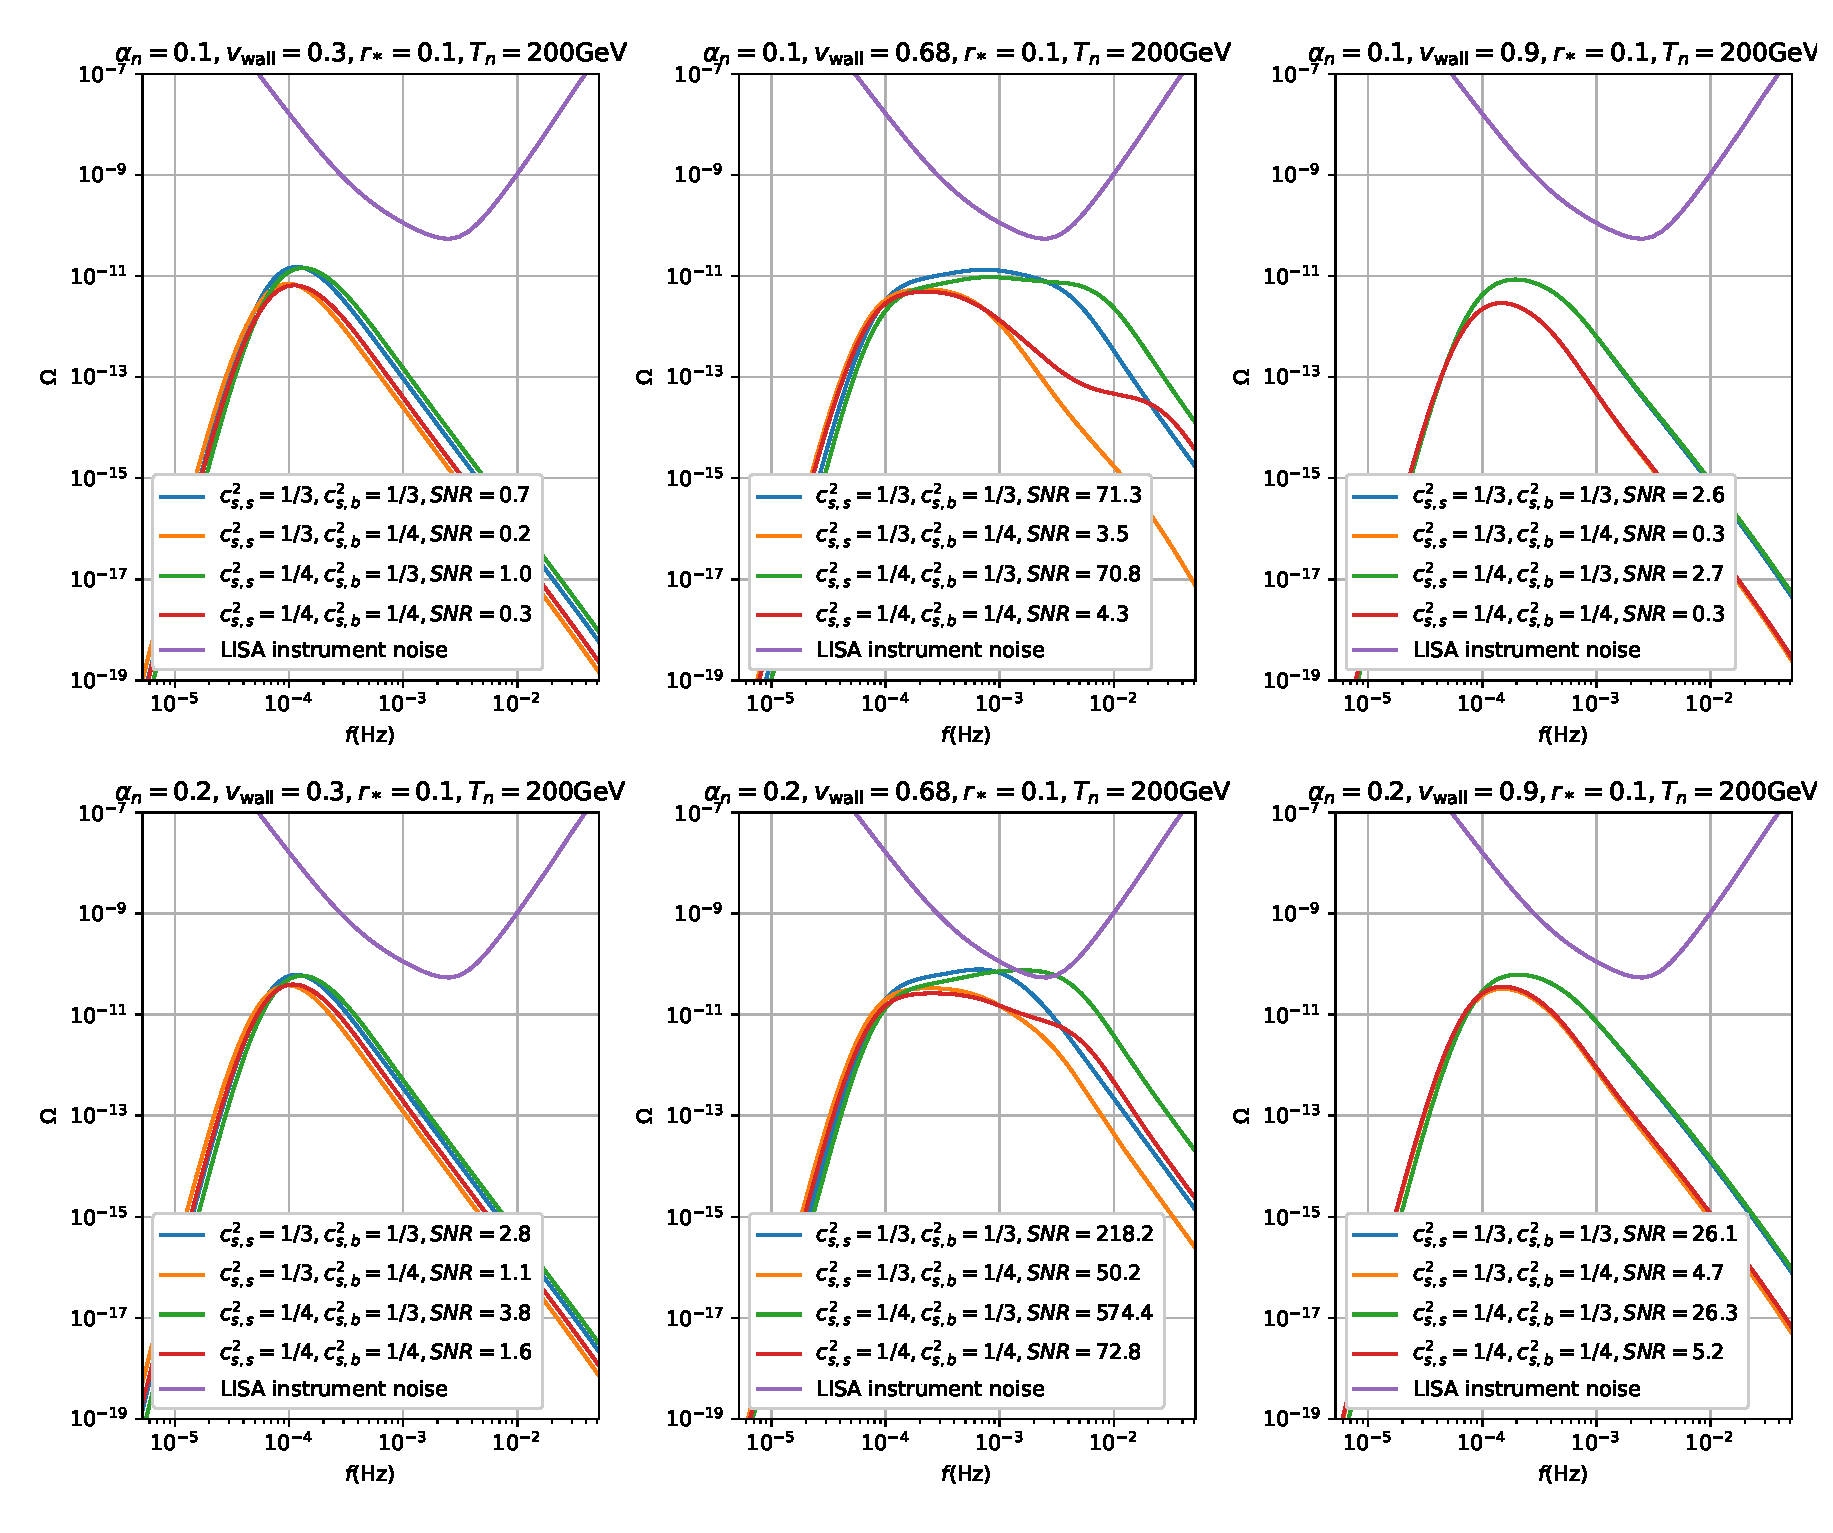
\includegraphics[width=\textwidth]{../pttools/examples/fig/const_cs_gw_omgw0.eps}
\caption{Gravitational wave power spectra today $\Omega_{gw,0}$}
\label{fig:omgw0}
\end{figure}

To test the precision and reliability of the results provided by PTtools,
we compared to the results in \cite[fig. 2]{giese_2021},
resulting in figure \ref{fig:kappa_giese}.
It should be noted that the article uses $\kappa_{\bar{\theta}_n}$ of eq. \eqref{eq:kappa_thetabar_n},
which differs from the $\kappa$ defined in eq. \eqref{eq:kappa_omega}.
The colors from blue to gray correspond to $\alpha = 0.01, 0.03, 0.1, 0.3, 1, 3$.
The figures on the left have $\alpha = \alpha_{\bar{\theta}_n}$
and the figures on the right have $\alpha = \alpha_n$.
For each color, the upper line has $c_{s,b}^2 = \frac{1}{3}$ and the lower line $c_{s,b}^2 = \frac{1}{4}$.
The solid lines correspond to $c_{s,s}^2 = \frac{1}{3}$ and the dashed lines correspond to $c_{s,s}^2 = \frac{1}{4}$.

\begin{figure}[h!]
\centering
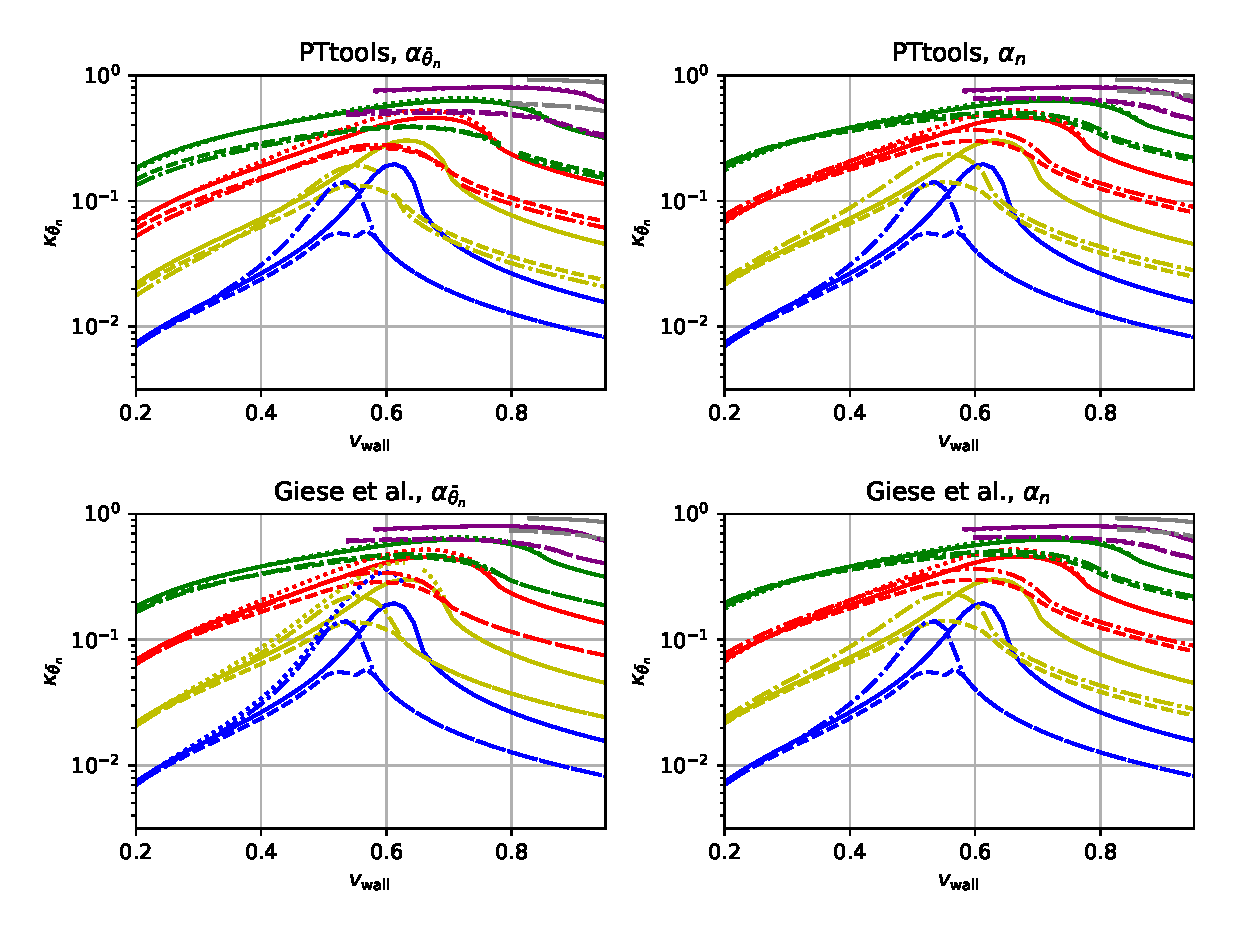
\includegraphics[width=\textwidth]{../pttools/examples/fig/giese_lisa_fig2.eps}
\caption{Comparison of $\kappa_{\bar{\theta}_n}$ values by \cite[fig. 2]{giese_2021} and PTtools}
\label{fig:kappa_giese}
\end{figure}
\todo{Use EPS instead of PNG}

It can be seen that PTtools and the code of \cite{giese_2021} produce results that are qualitativley similar, but slightly different.
This can be seen especially at the high wall speeds with $\alpha_n$ where changing $c_{s,s}$ (switching between the solid and dashed lines) has the opposite effect.

The gaps in the PTtools curves are caused by difficulties in finding a solution for very thin hybrid shells at the hybrid-detonation boundary.
It can happen that the shell is so thin that
It is also possible that the validity checks don't capture all the issues at this boundary,
resulting in a slightly wrong result.
This is demonstrated by the solid green $\alpha_n = 0.3, c_{s,s}^2 = \frac{1}{4}, c_{s,b} = \frac{1}{4}$ curve in the top-right figure.
These issues continue to be under investigation.

Some of the curves are not plotted by PTtools at all, since it has stricter tests for the validity of the bubble than the reference code.
One of such restrictions is that the $\alpha_n$ must be above the theoretical minimum for the model,
and that the model must have a valid critical temperature.
